% artikkel_III_form_og_tid.tex
% Artikkel III: Form og tid - dimensjonar, stil og prediksjon
% STOLAR-prosjektet - Kvantitativ designhistorie
% Spraak: Nynorsk

\documentclass[12pt, a4paper]{article}

\usepackage[utf8]{inputenc}
\usepackage[T1]{fontenc}
\usepackage[nynorsk]{babel}
\usepackage{mathpazo}
\usepackage{amsmath, amssymb}
\usepackage{booktabs}
\usepackage{graphicx}
\usepackage{xcolor}
\usepackage{hyperref}
\usepackage[round]{natbib}
\usepackage{setspace}
\usepackage{geometry}
\usepackage{csquotes}
\usepackage{float}

\geometry{margin=2.5cm}
\onehalfspacing
\graphicspath{{fig/}}

\title{%
  \textbf{Form og tid}\\[0.4em]
  \large Maskinl\ae ring, teknikk-entropi og det emergente stilomgrepet%
}
\author{%
  Iver Raknes Finne\\
  \small Arkitektur- og designhøgskolen i Oslo (AHO)\\
  \small \texttt{iver.raknes.finne@stud.aho.no}
}
\date{}

\begin{document}
\maketitle

% ================================================================
\begin{abstract}
\noindent Stilperiodar (barokk, rokokko, funksjonalisme) vert tradisjonelt handsama som \emph{årsaker} til form: ein stol ser ut som han gjer \emph{fordi} han tilhøyrer ein stil. Denne artikkelen snur kausaliteten. Ved hjelp av \textbf{Random Forest}-klassifikasjon på 469 stolar med stilmerke frå STOLAR-databasen syner me at fire dimensjonsvariablar (høgde, breidde, djupn, setehøgde) og 30 binære materialkodar predikerer stilperiode med $F1 = 0{,}823$. Dimensjonar åleine gjev $F1 = 0{,}777$; materialar åleine $F1 = 0{,}678$. Høgde er den viktigaste enkeltvariabelen (19,7\,\% av total feature importance). Samstundes syner ein parallell analyse at Shannon-entropien for \textbf{konstruksjonsteknikkar} stig frå 1,0 bits (1200-talet) til 3,67 bits (2000-talet), ein utvikling som speglar materialentropien frå Artikkel~I. Funna tyder at stilperiodar ikkje er diskrete kategoriar med kausal kraft, men \textbf{emergente merkelappar}: etterrasjonaliserte namn på klynger i eit fleiraksig formrom som er styrt av djupare krefter: dimensjonar, materialtilgang og produksjonsteknologi.

\medskip
\noindent\textbf{Nøkkelord:} maskinlæring, Random Forest, stilperiode, teknikk-entropi, feature importance, formprediksjon, kvantitativ designhistorie
\end{abstract}

\vspace{1em}
\hrule
\vspace{1.5em}


% ================================================================
\section{Innleiing: er stil ei årsak eller eit symptom?}

Designhistoria er organisert rundt stilperiodar: renessanse, barokk, rokokko, nyklassisisme, jugend, funksjonalisme, postmodernisme. Desse kategoriane strukturerer museum, lærebøker og kuratorpraksis. Men dei ber med seg ein implisitt kausal påstand: at stilen \emph{forklarer} forma. Ein stol er høg og ornamentert \emph{fordi} han er barokk. Ein stol er låg og geometrisk \emph{fordi} han er funksjonalistisk.

Men kva om kausaliteten går andre vegen? Kva om stilperiodar er \emph{etterpå-kategoriar}: namn me gjev til klynger av objekt som liknar kvarandre, utan at namnet har kausal kraft? I biologien skil ein mellom \emph{fenotyp} (den observerbare forma) og \emph{genotyp} (den underliggjande årsaka). Stilmerket er ein fenotypisk merkelapp, men dei underliggjande årsaka kan vere dimensjonar, materialtilgang og produksjonsteknikk.

Denne artikkelen, den tredje i serien, brukar maskinlæring for å teste kva variablar som ber mest informasjon om stil, og om stilmerket sjølv har prediktiv kraft.


% ================================================================
\section{Teoretisk bakgrunn}

\subsection{Stilomgrepet i designhistorie}

Stilperiodar har ei lang historiografisk historie. \citet{lucie-smith1993} og \citet{raizman2010} organiserer designhistoria kronologisk etter stilperiodar, der kvar periode vert definert av eit sett formtrekk: kurvede liner for rokokko, rette for nyklassisisme, organiske for jugend. Men som \citet{kuhn1962} minna om for vitskaplege paradigme, er kategoriane ofte meir stabile enn fenomena dei skal fange. Stilgrensene er uskarpe, overlappande og retrospektive.

\subsection{Maskinlæring som epistemisk verktøy}

\textbf{Random Forest} \citep{breiman2001} er ein ensemblemetode som byggjer mange avgjerdstrær og aggregerer prediksjonane deira. Styrken ligg i at modellen er \emph{ikkje-parametrisk}: han gjer ingen antakingar om funksjonell form mellom variablar. Dersom dimensjonar og materialar predikerer stilperiode med høg presisjon, tyder det at det eksisterer systematiske, maskinlærlege mønster i data som korresponderer med stilkategoriane. Feature importance gjev oss i tillegg eit rangert mål på kva variablar som bidreg mest til prediksjonen.

\subsection{Teknikk som formkraft}

Kvar konstruksjonsteknikk avlegg eit fysisk avtrykk i den ferdige stolen. \textbf{Tapping} (tapping av mortis-og-tenon-samanføyingar) krev massive tverrsnitt. \textbf{Formbøying} (til dømes Thonet sin dampbøygde bøk) mogeleggjer slanke, kurva profil. \textbf{Sveising} frigjer stål frå rette liner. \textbf{Sprøytestøyping} mogeleggjer amorfe plastformer. Teknikkrepertoaret i eit hundreår avgrensar formrommet i det hundreåret, på same vis som materialpaletten gjer det.


% ================================================================
\section{Metode}

\subsection{Klassifikasjon av stilperiode}

Me trenar ein \textbf{Random Forest}-klassifikator (100 trær, 5-faldig stratifisert kryssvalidering) til å predikere stilperiode frå:
\begin{enumerate}
  \item Fire dimensjonsvariablar: høgde, breidde, djupn, setehøgde.
  \item 30 binære materialkodar: dei mest frekvente materiala (kvar med $\geq 20$ førekomstar).
  \item Kombinasjonen av (1) og (2).
\end{enumerate}

Utvalet er $n = 469$ stolar med gyldige dimensjonar \emph{og} stilmerke. Berre stilperiodar med $\geq 10$ stolar er inkluderte ($k = 15$ stilar). Evalueringsmålet er \textbf{vekta F1-score} (gjennomsnittleg F1 vekta etter klassestorleik).

\subsection{Teknikk-entropi}

Me reknar ut Shannon-entropi ($H'$, i bits) for konstruksjonsteknikkar per hundreår, analogt med materialentropien i Artikkel~I. Teknikkar er registrerte som kommaseparerte felt (t.d. \texttt{Polstring, Tapping, Plugging}).


% ================================================================
\section{Resultat}

\subsection{Dimensjonar predikerer stilperiode}

\begin{table}[H]
\centering
\caption{Random Forest-klassifikasjon av stilperiode ($k = 15$ stilar, $n = 469$). Vekta $F1$, 5-faldig CV.}
\label{tab:rf_style}
\begin{tabular}{@{}lcc@{}}
\toprule
\textbf{Feature-sett} & \textbf{$F1$ (vekta)} & \textbf{$\pm\sigma$} \\
\midrule
Dimensjonar åleine (4 var.) & 0,777 & 0,036 \\
Materialar åleine (30 var.) & 0,678 & 0,032 \\
Dimensjonar + materialar (34 var.) & 0,823 & 0,036 \\
\bottomrule
\end{tabular}
\end{table}

\begin{figure}[H]
  \centering
  
\includegraphics[width=0.85\textwidth]{fig7_feature_importance.pdf}
  \caption{Feature importance for stilklassifisering (Random Forest). Dimensjonar (mork) dominerer med 56,7\,\% samla importance.}
  \label{fig:importance}
\end{figure}

Tre funn er sentrale:

\begin{enumerate}
  \item \textbf{Dimensjonar ber mest informasjon.} Fire metriske variablar ($F1 = 0{,}777$) predikerer stilperiode betre enn 30 materialkategoriar ($F1 = 0{,}678$). Forma sin geometri er ein sterkare stilmarkør enn materialvalet.

  \item \textbf{Kombinasjonen aukar presisjonen marginalt.} Å leggje til materialar aukar $F1$ frå 0,777 til 0,823: ein forbetring på 4,6 prosentpoeng. Materialar gjev tilleggsinformasjon, men dimensjonane gjer hovudarbeidet.

  \item \textbf{Høgde er den viktigaste enkeltvariabelen.} Feature importance-analysen (tabell~\ref{tab:importance}) viser at høgde åleine står for 19,7\,\% av total prediktiv kraft, følgd av breidde (14,0\,\%), djupn (12,0\,\%) og setehøgde (11,0\,\%). Dei fire dimensjonsvariablane utgjer 56,6\,\% av total importance, trass i at dei berre er 4 av 34 variablar.
\end{enumerate}

\begin{table}[H]
\centering
\caption{Topp 10 feature importance for stilperiode-prediksjon (Random Forest, 200 trær).}
\label{tab:importance}
\begin{tabular}{@{}rlr@{}}
\toprule
\textbf{Rang} & \textbf{Variabel} & \textbf{Importance} \\
\midrule
1 & Høgde & 0,197 \\
2 & Breidde & 0,140 \\
3 & Djupn & 0,120 \\
4 & Setehøgde & 0,110 \\
5 & Bøk & 0,038 \\
6 & Buksbom & 0,037 \\
7 & Mahogni & 0,036 \\
8 & Silke & 0,035 \\
9 & Hestetagl & 0,035 \\
10 & Messing & 0,023 \\
\bottomrule
\end{tabular}
\end{table}


\subsection{Nasjonalitet og hundreår}

Modellen predikerer òg nasjonalitet og hundreår med høg presisjon:

\begin{table}[H]
\centering
\caption{Random Forest-prediksjon av ulike målvariablar.}
\label{tab:rf_all}
\begin{tabular}{@{}llcc@{}}
\toprule
\textbf{Features} & \textbf{Mål} & \textbf{$F1$} & \textbf{$n$} \\
\midrule
Dim. + mat. & Stilperiode & 0,823 & 469 \\
Dim. + mat. & Nasjonalitet & 0,721 & 1\,231 \\
Dim. + mat. & Hundreår & 0,776 & $\sim$2\,000 \\
Stilmerke åleine & Hundreår & 0,799 & $\sim$400 \\
\bottomrule
\end{tabular}
\end{table}

Eit slåande funn: \textbf{stilmerket åleine predikerer hundreår med $F1 = 0{,}799$}, noko som tyder at stilperiodar er sterkt korrelerte med tid. Men dette er ikkje overraskande: stilmerke \emph{er} per definisjon tidsavgrensa kategoriar. Det interessante er at \emph{dimensjonar og materialar} ($F1 = 0{,}776$) nesten matcherer stilmerket sin prediksjon av hundreår, utan å ha tilgang til stilinformasjonen. Forma sjølv ber nesten like mykje tidsinformasjon som den eksplisitte stiletiketten.


\subsection{Dimensjonar per stilperiode}

Tabell~\ref{tab:style_dims} syner gjennomsnittlege dimensjonar for dei mest representerte stilperiodane, sortert etter høgde. Mønsteret er slåande: høgde fell monotont frå tidlege stilar (régence: 114,5 cm) til seine stilar (funksjonalisme: 77,7 cm).

\begin{table}[H]
\centering
\caption{Gjennomsnittlege dimensjonar per stilperiode (stilar med $n \geq 10$, sortert etter høgde).}
\label{tab:style_dims}
\begin{tabular}{@{}lrrrr@{}}
\toprule
\textbf{Stilperiode} & \textbf{$n$} & \textbf{$\bar{H}$ (cm)} & \textbf{$\sigma_H$} & \textbf{$\bar{W}$ (cm)} \\
\midrule
Régence & 27 & 114,5 & 7,6 & 49,5 \\
Barokk & 92 & 110,2 & 22,8 & 51,6 \\
Queen Anne & 12 & 106,1 & 3,4 & 50,1 \\
Renessanse & 18 & 101,9 & 17,9 & 66,4 \\
Rokokko & 27 & 97,9 & 4,6 & 49,3 \\
Louis XVI & 22 & 94,2 & 2,3 & 58,4 \\
Jugend & 21 & 94,1 & 7,4 & 48,7 \\
Hepplewhite & 28 & 93,2 & 1,5 & 50,4 \\
Historisme & 64 & 89,0 & 10,9 & 47,2 \\
Nyklassisisme & 26 & 85,4 & 7,9 & 48,1 \\
Modernisme & 17 & 84,2 & 12,6 & 53,5 \\
Empire & 36 & 80,8 & 1,1 & 46,5 \\
Funksjonalisme & 47 & 77,7 & 11,7 & 57,5 \\
\bottomrule
\end{tabular}
\end{table}

Denne tabellen forklarer kvifor dimensjonar predikerer stil så godt: det er ein \emph{kronologisk gradient} i høgde som samstundes er ein stilistisk gradient. Barokkstolen (110 cm) er fundamentalt ein annan fysisk gjenstand enn funksjonalisme-stolen (78 cm). Dei 32 centimetrane som skil dei er ikkje ornament: dei er strukturell endring i korleis stolen held kroppen.

\begin{quote}
\textbf{Stilens dimensjonale signatur:} Kvar stilperiode har ein karakteristisk dimensjonsprofil som er maskinlærleg distinkt. Men denne profilen er ikkje \emph{årsaka} av stilen: han \emph{er} stilen. Stilmerket er det menneskelege namnet me gjev til ein klynge i dimensjonsrommet. Det har ikkje meir kausal kraft enn namnet ``tropisk sone'' har over temperaturen.
\end{quote}


\subsection{Teknikk-entropi: formrommet sine verktøy}

Parallelt med material- og dimensjonsanalysen undersøkjer me korleis \textbf{konstruksjonsteknikkar} utviklar seg over tid.

\begin{table}[H]
\centering
\caption{Shannon-entropi ($H'$ i bits) for konstruksjonsteknikkar per hundreår.}
\label{tab:tech_entropy}
\begin{tabular}{@{}lrrrrll@{}}
\toprule
\textbf{Hundreår} & \textbf{$N$} & \textbf{$S$} & \textbf{$H'$} & \textbf{$J'$} & \textbf{Topp teknikk} \\
\midrule
1200-talet &    2 &  2 & 1,00 & 1,00 & Plugging, Tapping \\
1500-talet &   17 &  5 & 1,93 & 0,83 & Skjering \\
1600-talet &  385 & 11 & 2,98 & 0,86 & Skjering, Polstring \\
1700-talet &  773 & 20 & 2,77 & 0,64 & Polstring (38\,\%) \\
1800-talet &  456 & 20 & 2,98 & 0,69 & Polstring, Tapping \\
1900-talet &  433 & 29 & 3,64 & 0,75 & Polstring, Formbøying \\
2000-talet &   74 & 18 & 3,67 & 0,88 & Skruing, Formbøying \\
\bottomrule
\end{tabular}
\end{table}

\begin{figure}[H]
  \centering
  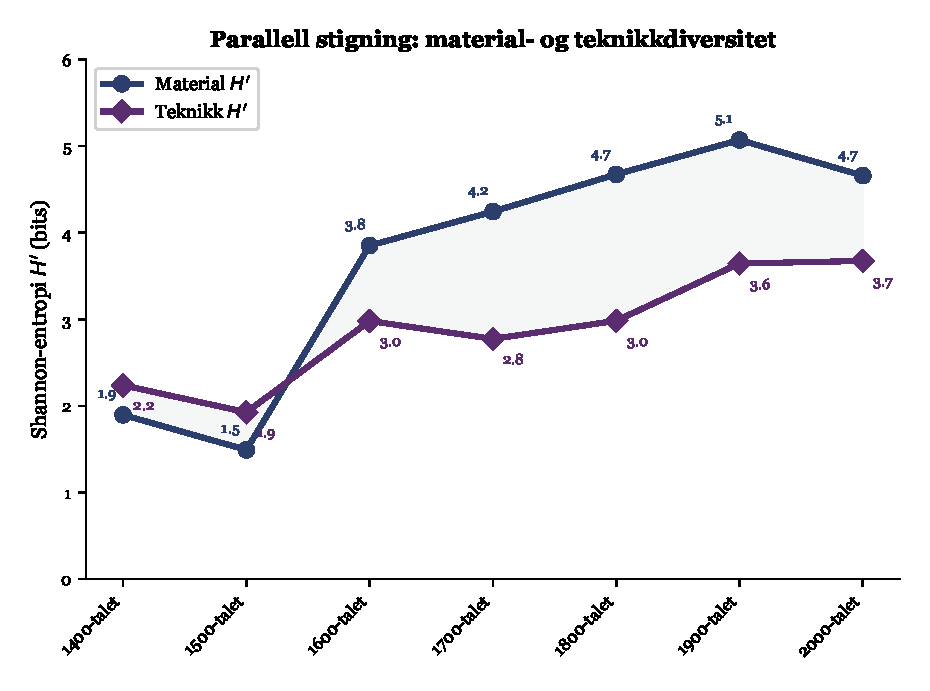
\includegraphics[width=0.9\textwidth]{fig8_teknikk_entropi.pdf}
  \caption{Parallell stigning: material- og teknikk-entropi over tid. Begge kurver stig fraa $\sim$1 bit til $\sim$4--5 bits.}
  \label{fig:teknikk}
\end{figure}

Teknikk-entropien stig frå 1,0 bits til 3,67 bits, ein parallell til materialentropien.

\begin{figure}[H]
  \centering
  
\includegraphics[width=\textwidth]{fig13_teknikk_evolusjon.pdf}
  \caption{Teknikk-evolusjon over fem hundreaar. Raude boksar markerer teknikkar som forsvinn (skjering, dreiing); gronne markerer teknikkar som oppstaar (formboyging, laminering, sveising).}
  \label{fig:teknikk_evo}
\end{figure} Nye teknikkar kumulerer: \emph{dreiing} kjem på 1500-talet, \emph{formbøying} og \emph{laminering} på 1800-talet, \emph{sveising} og \emph{sprøytestøyping} på 1900/2000-talet. Kvar ny teknikk opnar nye regionar i formrommet.

Eit interessant mønster dukkar opp på 1700-talet: jamnheita $J'$ fell til 0,64, den lågaste i heile serien. Polstring dominerer med 38\,\% av alle teknikk-førekomstar. Dette er eit \emph{teknikkmonopol} som speglar mahogni-monopolet i materialdata: ein dominerande teknikk som driv andre ut i periferien. Polstring og mahogni er ikkje uavhengige fenomen; dei er to sider av same koloniale stolparadigme: importert tre med polstra sete.

\subsubsection{Teknikkar som forsvinn og oppstår}

Figur~\ref{fig:teknikk_evo} avdekkjer ein dramatisk teknikk-suksesjon over fem hundreår:

\begin{itemize}
  \item \textbf{Skjering} fell frå 47\,\% av alle teknikkførekomstar på 1500-talet til under 1\,\% på 1900-talet. Handskjering er tidkrevjande og krev virtuos handverkskompetanse; ho vert marginalisert av maskinelle alternativ.
  \item \textbf{Dreiing} (dreiebenk) fell frå 18\,\% (1500-talet) til 15\,\% (1600-talet) og vidare til null etter 1800. Den dreia stolperamma, karakteristisk for barokken, forsvinn når nye samanbindingsteknikkar vert tilgjengelege.
  \item \textbf{Formbøying} dukkar opp frå null til 14\,\% på 1900-talet, driven av Michael Thonet sin dampbøyingsteknikk frå 1850-talet \citep{thonet1976}. Denne eine innovasjonen opna heile regionar av formrommet som tidlegare var utilgjengelege.
  \item \textbf{Skruing} stig frå 1\,\% (1700-talet) til 18\,\% (2000-talet), som reflekterer overgangen frå irreversible til reversible samanbindingar.
  \item \textbf{Sveising} og \textbf{sprøytestøyping} dukkar opp på 1900/2000-talet og representerer fundamentalt nye formgjevingsparadigme: metallsamanbinding utan kontakt og polymerforming utan verktøyavgrensing.
\end{itemize}

Kvar ny teknikk opnar ein ny region i formrommet. Formbøying mogleggjorde Thonet-stolen sin ikoniske kurva; sveising mogeleggjorde Breuer sin røyrstol; sprøytestøyping mogeleggjorde Panton sin heilstøypte plastkurve. Teknikken er ikkje ei implementeringsdetalj; ho er ein \emph{formgjevande kraft} som avgrensar og mogeleggjer geometriar.


\subsection{Material-teknikk-koplingane}

Tabell~\ref{tab:mat_tech} syner dei mest frekvente material-teknikk-para i heile databasen.

\begin{table}[H]
\centering
\caption{Topp 10 material-teknikk-par (heile perioden).}
\label{tab:mat_tech}
\begin{tabular}{@{}llr@{}}
\toprule
\textbf{Materiale} & \textbf{Teknikk} & \textbf{$n$} \\
\midrule
Bøk & Polstring & 224 \\
Mahogni & Polstring & 199 \\
Bøk & Tapping & 158 \\
Silke & Polstring & 134 \\
Hestetagl & Polstring & 124 \\
Nøttetre & Polstring & 107 \\
Tekstil & Polstring & 107 \\
Mahogni & Tapping & 100 \\
Furu & Polstring & 97 \\
Furu & Tapping & 89 \\
\bottomrule
\end{tabular}
\end{table}

Polstring dominerer koplingane: 7 av dei 10 mest frekvente para involverer polstring. Dette reflekterer polstring sin unike rolle som ein \emph{grensesnitt-teknikk}: han krev alltid eit berande trevirke (bøk, mahogni, furu) \emph{og} eit dekkmateriale (silke, tekstil, lær). Polstring er dermed ein koplar mellom materialverda og brukarverda, mellom den geopolitiske forsyningskjeda og kroppen som sit.


\subsection{Nasjonale dimensjonssignaturar}

\begin{table}[H]
\centering
\caption{Gjennomsnittleg stolhøgde per nasjonalitet (nasjonalitetar med $n \geq 10$).}
\label{tab:nat_dims}
\begin{tabular}{@{}lrrrr@{}}
\toprule
\textbf{Nasjonalitet} & \textbf{$n$} & \textbf{$\bar{H}$ (cm)} & \textbf{$\sigma_H$} & \textbf{$\bar{W}$ (cm)} \\
\midrule
Noreg & 153 & 98,2 & 23,3 & 51,4 \\
Austerrike & 18 & 88,6 & 45,7 & 56,7 \\
Storbritannia & 773 & 83,6 & 58,2 & 62,4 \\
Italia & 96 & 83,4 & 33,0 & 58,8 \\
Danmark & 48 & 74,9 & 22,9 & 56,6 \\
Frankrike & 109 & 74,4 & 28,0 & 61,2 \\
Tyskland & 44 & 72,8 & 23,6 & 58,1 \\
Finland & 22 & 62,1 & 23,1 & 56,3 \\
\bottomrule
\end{tabular}
\end{table}

Kvar nasjon har ein distinkt dimensjonsprofil. Norske stolar (98,2 cm) er i snitt 36,1 cm høgare enn finske (62,1 cm). Denne skilnaden reflekterer ikkje ulike menneskekroppar (nordmenn og finnar er om lag like høge), men ulike design- og materialkulturar: den norske tradisjonen med høge stolryggar i lokal eik og ask vs. den finske tradisjonen (dominert av Aalto og etterfølgjarane) med låge, bøygde bjørkekonstruksjonar.


% ================================================================
\section{Diskusjon}

\subsection{Stilperiodar som emergente kategoriar}

Hovudfunnet er at dimensjonar og materialar predikerer stilperiode med $F1 = 0{,}823$: ein maskinlæringsmodell kan klassifisere ein stol sin stilperiode med over 82\,\% presisjon berre basert på fire mål og 30 materialkategoriar. Men dette tyder \emph{ikkje} at stil er ei årsak. Det tyder at stil er eit \emph{emergent mønster}: ein klynge i formrommet som menneskelege observatørar har gjeve eit namn.

Analogen til biologien er instruktiv. Ein paleontolog kan klassifisere ein fossil etter art basert på dimensjonar og beinsstruktur med høg presisjon. Men det er ikkje \emph{artsnamnet} som skapar beina: det er dei underliggjande evolusjonære kreftene (seleksjon, drift, migrasjon) som skapar både forma og den klyngestrukturen me kallar ``art''. På same vis er det ikkje ``barokk'' som skapar høge stolryggar: det er materialøkologien (nøttetre, eik), produksjonsteknologien (skjering, dreiing) og den kulturelle konteksten (maktdemonstrasjon, komfort) som saman skaper den geometrien me etterpå kallar ``barokk''.

\subsection{Den kronologiske dimensjonsgradienten}

Tabell~\ref{tab:style_dims} avdekkjer ein slåande kronologisk gradient: stilperiodar som tilhøyrer tidlegare hundreår har konsekvent høgare stolar. Régence-stolar (114,5 cm) er 37 cm høgare enn funksjonalisme-stolar (77,7 cm). Denne gradienten er ikkje ornamental: han reflekterer ein strukturell endring i korleis stolen held kroppen. Barokkstolen med sin høge rygg og stolperamme er fundamentalt ein annan fysisk gjenstand enn funksjonalismestolen med sin låge, ergonomisk tilpassa profil.

Det er denne gradienten Random Forest-modellen fangar opp. Stilklassifisering er, i essens, høgdeklassifisering: ein maskin som kan gjette høgda, kan gjette stilen. Men dette betyr \emph{ikkje} at stilen forklarer høgda: det betyr at begge er uttrykk for same underliggjande krefter (materiale, teknikk, kulturell kontekst).

\subsection{Nasjonale dimensjonssignaturar og materialkoding}

Tabell~\ref{tab:nat_dims} syner at kvar nasjon har ein distinkt dimensjonsprofil. Norske stolar (98,2 cm) er 36 cm høgare enn finske (62,1 cm). Denne skilnaden reflekterer ikkje ulike menneskekroppar: nordmenn og finnar er tilnærma like høge. Han reflekterer ulike \emph{materialøkologiar} og \emph{designkulturar}.

Den finske lavmæla profilen er dominert av Alvar Aalto og etterfølgjarane hans: dampbøygd bjørk i slanke, låge konstruksjonar. Den norske høge profilen reflekterer ein barokk- og empiretradisjon med massive stolperammer i eik og mahogni. Materialet dikterer ikkje berre proporsjonen ($H/W$), men òg den absolutte dimensjonen: massive treslag krev massive konstruksjonar.

\subsection{Dimensjonane si forklaringskraft}

At fire metriske variablar åleine gjev $F1 = 0{,}777$ er eit sterkt funn. Det tyder at mesteparten av stilinformasjonen er koda i den fysiske geometrien, ikkje i materialvalet. Høgde er den viktigaste enkeltvariabelen (19,7\,\% importance). Dette svarar til funnet i Artikkel~II om den monotone høgdereduksjonen over tid: kvar epoke har sitt karakteristiske høgdeband, og dette bandet er den sterkaste prediktoren for stilperiode.

\subsection{Teknikk-entropi og formrommet}

Teknikk-entropien si parallelle stigning med materialentropien (begge frå $\sim$1 bit til $\sim$3,7 bits) er ikkje tilfeldig. Nye materialar krev nye teknikkar, og nye teknikkar mogeleggjer nye former. \emph{Formbøying} var umogleg før Thonet si dampbøying av bøk (1850-talet); \emph{sprøytestøyping} var umogleg før polymerindustrien (1960-talet). Kvar teknikk opnar ein ny region i formrommet, og det er desse regionane Random Forest-modellen navigerer når han predikerer stil.

\subsection{Avgrensingar}

Stilmerke er berre tilgjengelege for 22,9\,\% av utvalet ($n = 524$), noko som avgrensar den statistiske krafta. Klassifikasjonen er avhengig av kuratorens tildeling av stilmerke, som ikkje er standardisert. Feature importance frå Random Forest er eit relativt mål, ikkje eit kausalt mål. Modellen fangar korrelasjonar, ikkje årsakssamanhengar.


% ================================================================
\section{Konklusjon}

Dimensjonar og materialar kodar stil. Men stil kodar ikkje dimensjonar. Denne asymmetrien er det sentrale funnet: formrommet bestemmer kva klynger som oppstår, og stilmerka er dei menneskelege namna me gjev til desse klyngene. Å forklare ein stol sin form med referanse til stilperioden hans er ein sirkelargumentasjon: stilen \emph{er} forma, ikkje årsaka til henne.

Parallelt stig teknikk-entropien i takt med materialentropien. Formrommet utvidar seg langs tre aksar samstundes: fleire materialar, fleire teknikkar, fleire geometriar. Kvar akse forsterkar dei andre. Denne kumulative ekspansjonen av formrommet er den djupaste drivkrafta bak det me i ettertid kallar ``stilutvikling''.

Den neste og siste artikkelen i serien vil samle evidensen frå dei tre føregåande artiklane og formulere eit alternativt rammeverk: \emph{Form Follows Fitness}.


% ================================================================
\section*{Takk}

Takk til Nasjonalmuseet og Victoria and Albert Museum for open tilgang til samlingsdata.


% ================================================================
\bibliographystyle{plainnat}
\bibliography{references}

\end{document}
